%# -*- coding: utf-8-unix -*-
%%==================================================
%% chapter06.tex for SJTU Master Thesis
%%==================================================

%\bibliographystyle{sjtu2}%[此处用于每章都生产参考文献]
\chapter{多模态深度学习算法}
\label{chap:chap6}

\section{多模态深度学习介绍}
	随着近些年个人计算机计算能力的显著提高,Hinton提出的深度学习也越来越受到机器学习研究者的青睐。譬如在图像和文本领域,深度学习在图像识别和文本分类等任务中都表现的令人满意。然而随着图像和文本这两个模态的信息伴随彼此而一起出现的情况与日俱增(譬如微博的图片和文本),如何利用图像和文本之间的匹配关系,挖掘出他们的共有信息成为了多模态深度学习的目标。部分已有研究(需要加注释,引用)对图像和文本的多模态深度学习已经有了比单一模态的深度学习显著优秀的结果。因此,本课题就是在利用多模态的信息来进一步提升情绪识别的效果。本文利用EEG数据和眼动仪数据作为两个模态的输入,尝试寻找两者的匹配关系,并构建共有特征表达,虽然EEG数据和眼动仪数据两者不但在量级还是特征维度上的差别都十分巨大,但是我们仍旧达到比单一使用任意一个模态进行深度学习更好的效果。
	
\section{算法模型}
	我们的目的是设计合适的网络能够接受两个模态的输入,而输出两个模态的共有特征。自然的,我们选用深度神经网络(Deep Neural Network,简称DNN)作为基本框架。不过传统的DNN都是针对单模态的,于是,我们构建了以受限波尔兹曼机(Restricted Boltzmann Machines,简称为RBM)为基本单位的,多层次的多模态DNN。它可以接受两个模态的输入,并进行编码和解码过程,最终解码过后可以得到重建后的两个模态的特征。此时我们对重建后的特征和输入特征进行对比并且校正,多次迭代DNN网络就可以得到合适的网络参数,并且可以提取出网络中任意层次的共有特征表达。
	\subsection{RBM介绍}
	如果要进行深度学习的研究,那么必须要理解RBM的相关背景。\\
	\par
	\centerline{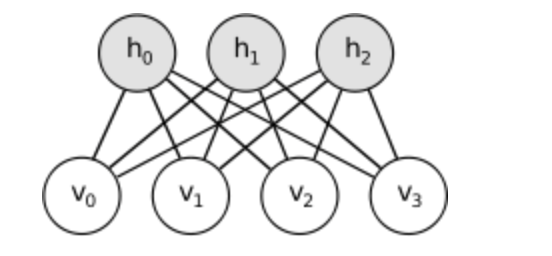
\includegraphics[width=4.5in]{figure/rbm.png}} %要居中就用centerline,这里的图片和tex 文件在一个目录下
	\centerline{图6-1}

	这是RBM的基本模型,其中v代表显层(visual), h代表隐层(hidden)。每个RBM都由一个显层和一个隐层组成,显层和隐层都可以有大于等于一的任意多个维度。而显层之间的所有单元均不相连,隐层之间的所有单元也全不相连。而两层之间的单元全相连。值得一提的是,如果所有单元保持全相连,那么这个模型就是波尔兹曼机(Boltzmann Machine),由于计算复杂度等原因,深度学习研究者通常使用RBM来构建深度网络。
	RBM是一个基于能量的模型(Energy-Based model),众所周知,一个基于能量的概率模型的概率分布由它独有的能量函数定义。对于常用的伯努利RBM来说,它的能量函数如下:
	\begin{equation}
	\begin{cases}
	E(s) = -\sum\limits_{i=1}^{n-1}\sum\limits_{j = i + 1}^{n} w_{ij}s_is_j - \sum\limits_{i=1}^n \theta_i s_i \\
	p(x) = \frac{e^{-E(x)}}{\sum\limits_t e^{-E(t)}}
	\end{cases}
	\end{equation}
	其中$s \in {0, 1}^n$  为n个单元的状态向量。 $w_{i, j}$ 为第i个和第j个单元之间的连接权,$\theta_i$为第i个单元的阈值。
	若网络中的神经元以任意不依赖输入值的顺序来更新,那么最终达到boltzmann,则训练完毕。
	具体更新过程如下:
	\begin{equation}
	\begin{cases}
	P(v|h) = \prod\limits_{i=1}^d P(v_i |h)\\
	P(h|v) = \prod\limits_{j=1}^q P(h_j |v)\\
	\end{cases}
	\end{equation}
	
	\begin{align}
	\Delta w = \eta(vh^T - v\prime {h\prime}^T)
	\end{align}
	然而由于伯努利RBM只允许显层和隐层的阈值在0,1之间,并且进行抽样更新的过程只能是1或者0。而我们的数据是在实数集上,虽然我们可以对数据进行针对每一维的归一化,从而让伯努利RBM变得可行,但是经过多次试验,我发现不同的归一化方法会产生各不相同的最终结果。为了解决这个这个问题,高斯RBM是一个不错的解决方法。它与伯努利RBM的区别在于更新过程和能量函数的计算。以下是它的具体计算方法:
	\begin{equation}
	E(v,h | \theta) = \sum\limits_{i=1}^{n_v}\frac{(v_i - b_i)^2}{2\sigma_i^2} - \sum\limits_{i=1}^{n_v}\sum\limits_{j=1}^{n_h} W_{i,j}h_j\frac{v_i}{\sigma_i} - \sum\limits_{j=1}^{n_h}c_jh_j
	\end{equation}
	
	\begin{equation}
	\begin{cases}
	P(v_i = v|h) = \mathcal{N}(v | b_i + \sum\limits_{j}h_jW_{ij}, \sigma^2)\\
	P(h_j = 1|v) = sigmoid(c_j + \sum\limits_i W_{ij} \frac{v_i}{\sigma_i^2})
	\end{cases}
	\end{equation}
	
	在根据隐层更新显层的过程中,需要根据b(显层阈值)和$\sigma_i$来确定这个神经元的高斯分布,再进行抽样。根据均值和标准差确定分布,获得抽样。
	
	在根据显层更新隐层的过程中,根据c(隐层阈值) 来确定伯努利分布,再进行抽样。 均值也就是$p(h_j| V)$, 根据这个值来确定分布,进行抽样。
	
	RBM的训练过程就是多次抽样和更新的过程。这也是一个马尔科夫链(Markov Chain)收敛的过程,每一步都是吉布斯采样(Gibbs Sampling)。吉布斯采样是用来构造多变量概率分布的随机样本的方法,特别常用于期望很难计算出来,而条件概率比较容易的得到的情况。
	
	N个元素的联合分布的吉布斯采样过程如下:每次分别对于一个元素采样,总共采样N次,就得到一个样本。具体算法如下:
	
	initialize $x_i$ : i = 1, 2, …, n, T samples:
	
	for t in range(1, T):\\

	\begin{equation}
	\begin{cases}
		x_1^{(t+1)} \sim p(x_1 | x_2^t, x_3^t,…, x_n^t)\\
		x_2^{(t+1)} \sim p(x_2 | x_1^({t+1)}, x_3^t,…, x_n^t)\\
		……\\
		x_j^{(t+1)} \sim p(x_j | x_1^{(t+1)},…,x_{(j-1)}^{(t+1)},x_{(j+1)}^t,…, x_n^t)\\
		……\\
		x_n^{(t+1)} \sim p(x_n | x_1^{t+1}, x_2^{t+1},…, x_{(n-1)}^{t+1})\\
	\end{cases}
	\end{equation}
	
	利用高斯RBM我们取得了比伯努利RBM更好的结果。
	\\
	\\
	\subsection{模型I}
		\centerline{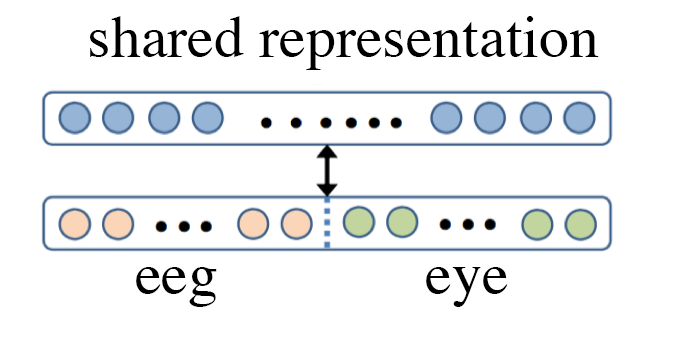
\includegraphics[width=4in]{figure/model1.png}} 
		\centerline{图6-2}
	
	如图所示,这个算法模型的功能是接受两个模态的输入,提取出两个模态的共同特征表达并输出。它的输出可以放到其他分类器,譬如SVM,神经网络等。这是一种比较直观,简单易懂的方法。那就是首先把眼动仪数据(图中eye)和脑电数据(图中eeg)直接进行拼接,两者时间窗口相同,数据也同时采集,所以样本数量相同。设眼动仪数据每个样本有n维,而脑电数据每个样本有m维,那么此时把它们拼接,得到(m + n)维的向量作为每个样本的特征。然后利用预训练之后的RBM进行特征提取,就得到了脑电数据和眼动仪数据的共同特征表达。
	
	然而,这个模型的缺点十分明显,就是这并不是一个深度的学习器,而是一个只有一层的网络,隐层和显层是线性连接的,所以这个模型很难找到眼动仪数据和脑电数据的非线性关系,并不能提取出理想的共同特征。
	
	为了解决这个问题,只能构建更深层次的网络。	
	\subsection{模型II}
		\centerline{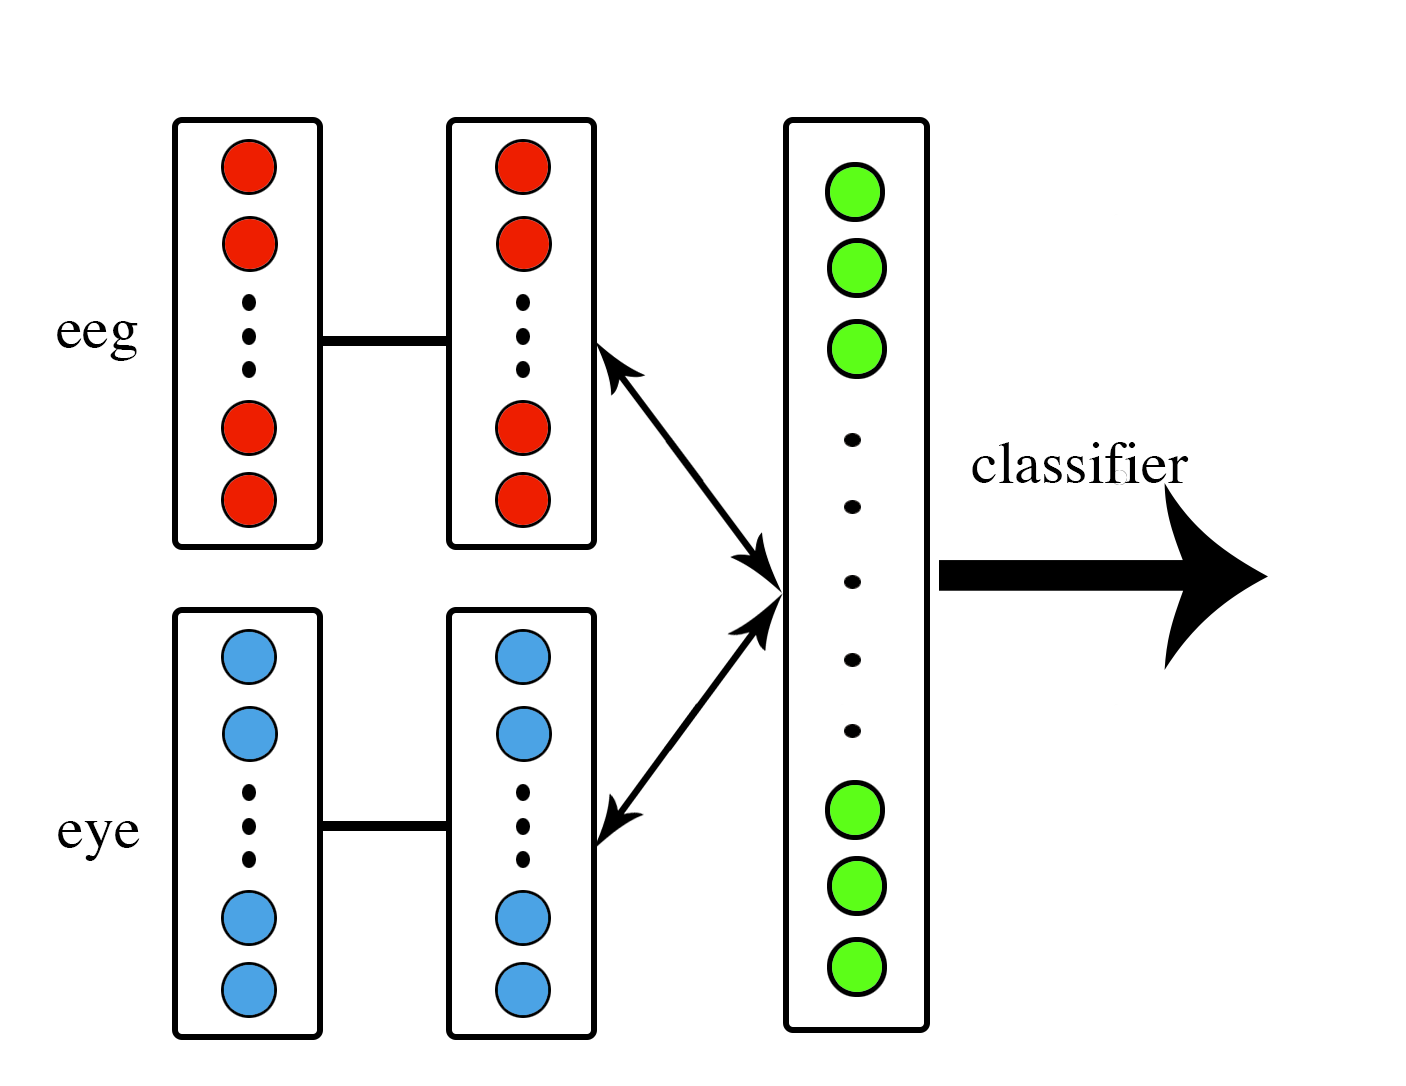
\includegraphics[width=5in]{figure/classify1.png}}
		\centerline{图6-3}
		如上图所示,此算法模型的功能与模型I类似,只是更加复杂,它可以更好的学习到两个模态的数据之间的非线性关系。首先用两个RBM分别提取眼动仪模态和脑电模态的特征,然后再将提取后的特征拼接,并再加一层网络提取共同表达的特征。这个网络一共包含三个RBM,在经过预训练和调参之后,我们获得了比模型I更好的结果。
		
		值得一提的是,模型I与模型II中每个RBM我们尝试了伯努利RBM和高斯RBM,然而在后续工作中我们发现在每个RBM的每个元素中都使用修正线性单元(Rectified Linear Unit,简写为ReLu)替代了sigmoid unit之后,便不再需要预训练,因此这个问题也就无需再考虑,因为不论是从速度还是结果来看,前者都是更优秀的。下文中将对这两个激活函数进行更详尽的对比。
	\subsection{模型III}
		\centerline{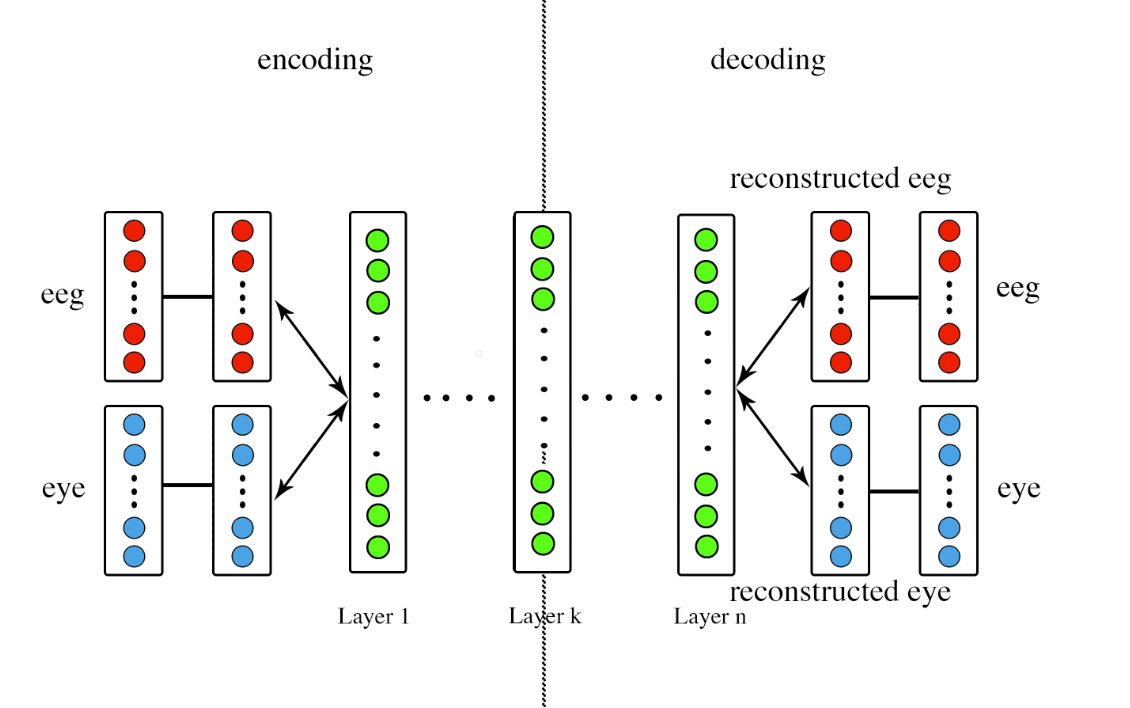
\includegraphics[width=7in]{figure/feature_learning.png}}
		\centerline{图6-4}
		
		如上图,这就是本文构建的特征提取算法模型。与前两个模型一样,它也接受两个模态的输入,并输出共同特征表达,用于后续的情绪识别任务。
		
		这个算法模型的左边是输入,右边是计算结果。我们把整个特征提取过程的一次迭代分成两个部分,左边半部分是编码过程(encoding),右边半部分是解码过程(decoding)。编码过程和解码过程应该是完全对称的,编码过程是学习更深层次特征的,解码过程是重建数据的。本模型首先分别对两个模态用RBM提取特征,然后对提取后的特征进行拼接,再加上k层网络增加深度来学习两个模态的非线性关系。图片中间的一层是编码的最后一层,也是解码的第一层。整个模型越靠中间的层,深度越深,也就代表了越抽象的特征,越靠近两边的层深度越浅,也就代表了越具体的特征。当计算到最右边一层的重建特征时,我们把整个特征向量一分为二,重新变为脑电数据和眼动仪数据两个模态,然后用输入数据和网络重建的数据进行对比,计算方差来校正整个网络的参数。 注意,即使最左边是数据输入,网络看似越靠右的层有越抽象,越深层次的特征,但是由于我们网络和更新算法的定义,编码过程里面才是越靠右的层越抽象的,而解码过程里面越靠右的层有越具体的特征,因为整个解码过程都在重建原本的特征,所以是不断变的更加具体的。
		
		然而,不像图像识别任务一样,深度网络的每个层次的特征都代表明确的意义,譬如浅层可能是直线和曲线,深层就是复杂的轮廓。趋势是越浅层的越局部越具体,越深层的越广泛越抽象。脑电和眼电数据的深度学习网络里,每个层次的数据并没有明确的意义。为了找出哪个层次的共同特征表达最适用于我们的情绪分类任务,我把从第一层到第n层的共同特征全部提取出来,并进行试验,得到了最终的结果。示意图见下方:
		\centerline{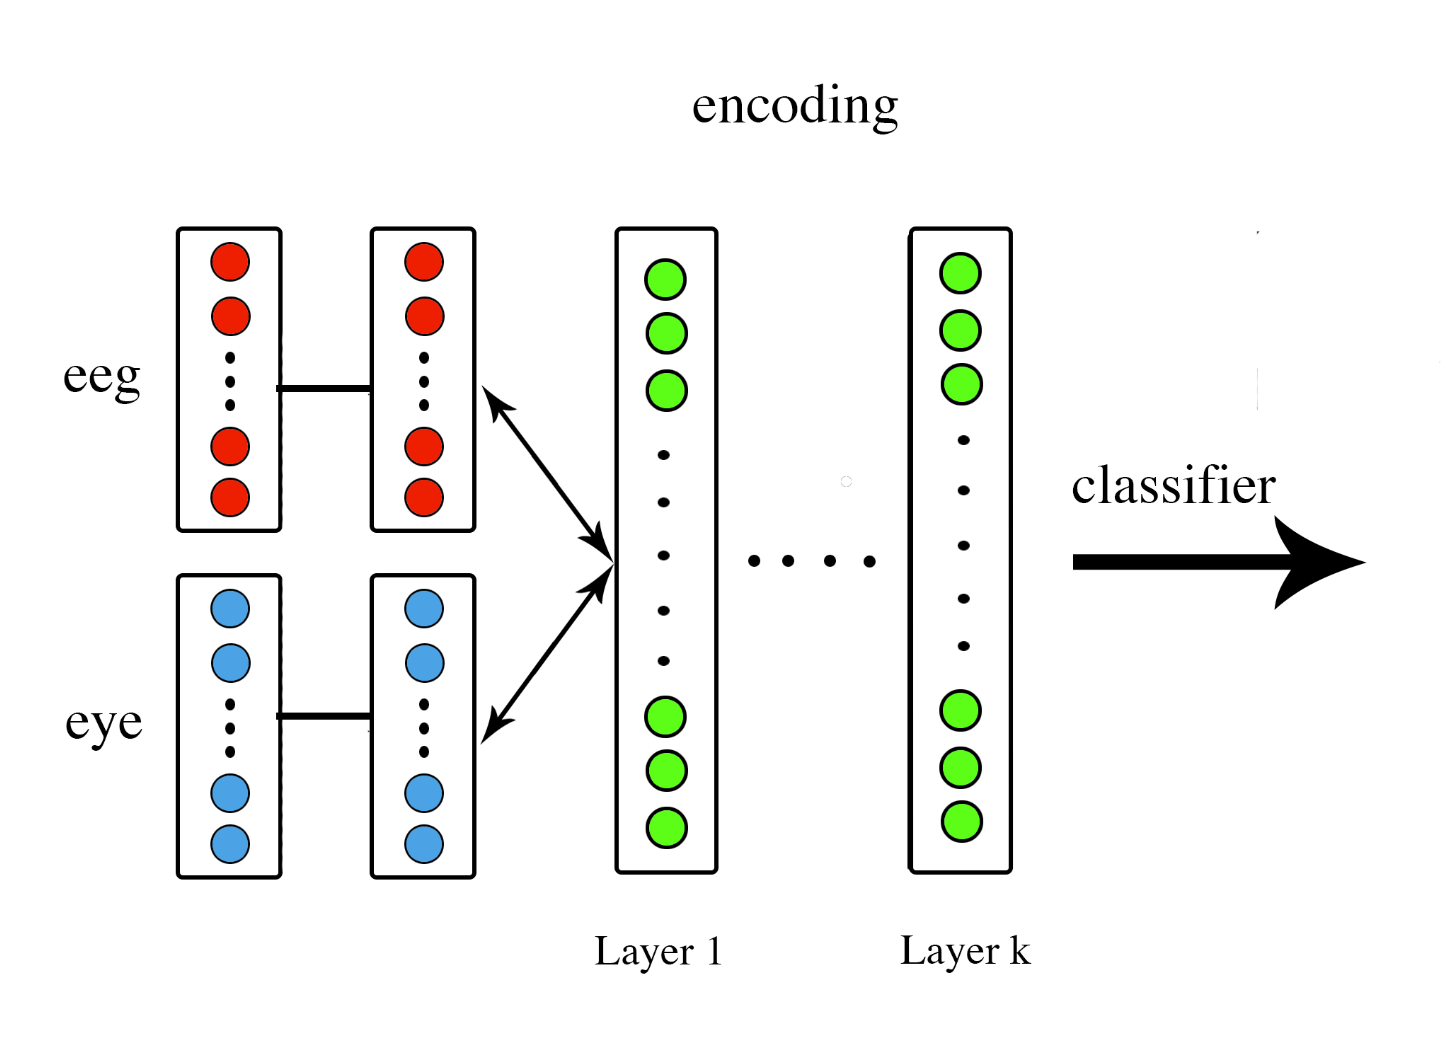
\includegraphics[width=5in]{figure/classifyk.png}}
		\centerline{图6-5}
		\centerline{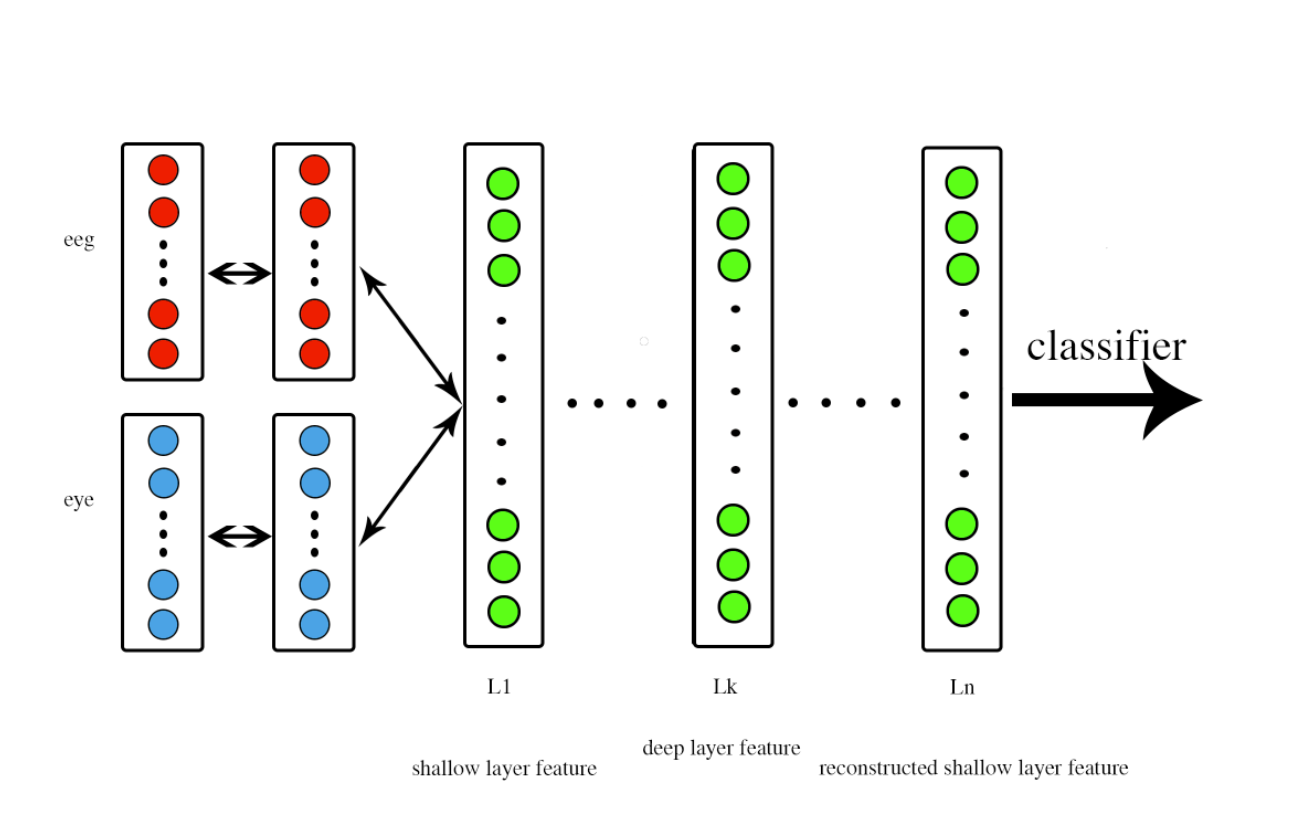
\includegraphics[width=5in]{figure/classifyn.png}}
		\centerline{图6-6}
		
		\centerline{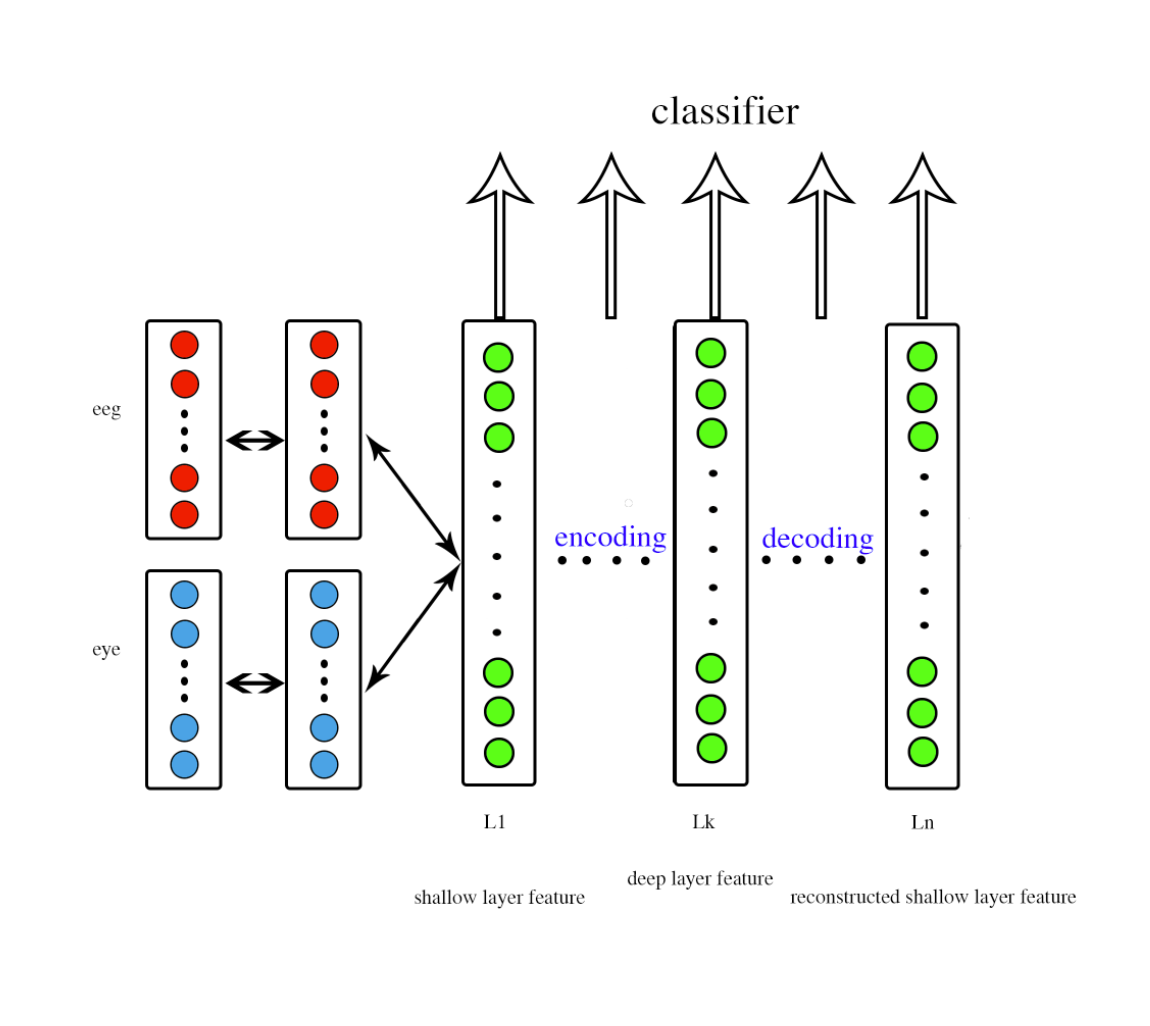
\includegraphics[width=5in]{figure/classify_all.png}}
		\centerline{图6-7}